%\subsection{Introduction}
\subsection{Types of Correlations}

\begin{figure}[ht]
    \centering

\includegraphics[scale=0.4]{choco-nobel}
\caption[Chocolate consumption and Nobel prizes]{Correlation between chocolate consumption and Nobel prizes \cite{Mes12}.}
%\footnotemark} 
\label{fig:choco-nobel}
\end{figure}

%\footnotetext{F.H. Messerli. \emph{Chocolate Consumption, Cognitive Function, and Nobel Laureates}. N Engl J. Med 2012; 367:1562-1564; DOI:10.1056/NEJMon1211064.} 


\begin{Expl}
    What conclusions can we make from this? Where does the correlation come from? Would the correlation hold under different conditions/circumstances?
    There are several explanations/stories that one could build around the measured correlation between the number of Nobel prizes $N$ and the chocolate consumption per capita $C$:
    \begin{enumerate}[label=\alph*)]
        \item $N$ causes $C$: ``Nobel prize winning countries like to celebrate with chocolate consumption.''
        \item $N$ is an effect of $C$: ``Chocolate contains brain enhancing chemicals.''
        \item Feedback between $N$ and $C$: Both stories hold.
        \item Selection bias between $N$ and $C$: ``$N$ and $C$ are actually independent, but the data used was biased, e.g.\ only Western and Asian countries were considered. Other countries might just be in the upper left or bottom right corners.''
        \item Functional constraints between $N$ and $C$: ``International regulations make sure that Nobel prizes and chocolate imports are subtracted/added if they violate a linear relationship.''
        \item $N$ and $C$ are confounded: ``The wealth of a country determines both, how much money goes to science and also how much people can spend on chocolate.''
        \item Other explanations, e.g.\ measurement error, statistical coincidence, other forms of spurious correlations, combinations of all of these, etc.?
    \end{enumerate}
\end{Expl}



\begin{figure}[ht]
    \begin{subfigure}[b]{.32\textwidth}
    \centering
    \begin{tikzpicture}[scale=1, transform shape]
        \tikzstyle{every node} = [draw,shape=circle,color=blue]
        \node (N) at (0,0) {$N$};
        \node (C) at (3,0) {$C$};
        \draw[-{Latex[length=3mm, width=2mm]}, color=blue] (N) to (C);
    \end{tikzpicture}
    \subcaption{}
    \label{subfig:N-causes-C}
    \end{subfigure}
    \begin{subfigure}[b]{.32\textwidth}
    \centering
    \begin{tikzpicture}[scale=1, transform shape]
        \tikzstyle{every node} = [draw,shape=circle,color=blue]
        \node (N) at (0,0) {$N$};
        \node (C) at (3,0) {$C$};
        \draw[-{Latex[length=3mm, width=2mm]}, color=blue] (C) to (N);
    \end{tikzpicture}
    \subcaption{}
    \label{subfig:N-effect-C}
    \end{subfigure}
    \begin{subfigure}[b]{.32\textwidth}
    \centering
    \begin{tikzpicture}[scale=1, transform shape]
        \tikzstyle{every node} = [draw,shape=circle,color=blue]
        \node (N) at (0,0) {$N$};
        \node (C) at (3,0) {$C$};
        \draw[-{Latex[length=3mm, width=2mm]}, color=blue, bend left] (N) to (C);
        \draw[-{Latex[length=3mm, width=2mm]}, color=blue, bend left] (C) to (N);
    \end{tikzpicture}
    \subcaption{}
    \label{subfig:N-feedback-C}
    \end{subfigure}

    \begin{subfigure}[b]{.32\textwidth}
    \centering
    \begin{tikzpicture}[scale=1, transform shape]
        \tikzstyle{every node} = [draw,shape=circle,color=blue]
        \node (N) at (0,0) {$N$};
        \node (C) at (3,0) {$C$};
        \tikzstyle{every node} = [draw,shape=circle,color=black, fill=green]
        \node (S) at (1.5,-2) {$S$};
     %   \draw[-{Latex[length=3mm, width=2mm]}, color=blue] (N) to (C);
        \draw[-{Latex[length=3mm, width=2mm]}, color=green] (N) to (S);
        \draw[-{Latex[length=3mm, width=2mm]}, color=green] (C) to (S);
    \end{tikzpicture}
    \subcaption{}
    \label{subfig:N-selection-bias-C}
    \end{subfigure}
    \begin{subfigure}[b]{.32\textwidth}
    \centering
    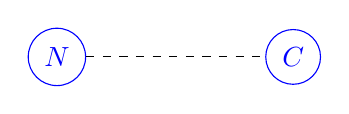
\begin{tikzpicture}[scale=1, transform shape]
        \tikzstyle{every node} = [draw,shape=circle,color=blue]
        \node (N) at (0,0) {$N$};
        \node (C) at (3,0) {$C$};
        \draw[-, dashed, color=black] (N) to (C);
    \end{tikzpicture}
    \subcaption{}
    \label{subfig:N-constrained-C}
    \end{subfigure}
    \begin{subfigure}[b]{.32\textwidth}
    \centering
    \begin{tikzpicture}[scale=1, transform shape]
        \tikzstyle{every node} = [draw,shape=circle,color=blue]
        \node (N) at (0,0) {$N$};
        \node (C) at (3,0) {$C$};
        \tikzstyle{every node} = [draw,shape=circle,color=red]
        \node (W) at (1.5,2) {$W$};
      %  \draw[-{Latex[length=3mm, width=2mm]}, color=blue] (N) to (C);
        \draw[-{Latex[length=3mm, width=2mm]}, color=red] (W) to (N);
        \draw[-{Latex[length=3mm, width=2mm]}, color=red] (W) to (C);
    \end{tikzpicture}
    \subcaption{}
    \label{subfig:N-confounded-C}
    \end{subfigure}
    \caption{Graphical representations of different correlation inducing scenarios.}
    \label{fig:choco-nobel-graph}
\end{figure}


\begin{Disc}
    Correlation does not imply causation because there are other possible correlation inducing scenarios.
    Also, correlation is symmetric, causation is asymmetric.
\end{Disc}

%\begin{Exc}
%    Go through the news articles that claim statements like "drinking wine every day improves your health", etc., and look up the study and 
%\end{Exc}


